
\chapter{Speaker Diarization in Co-channel Speech}
\label{chap:spkr_diar}

Throughout the course of this study, part of the agenda has been to acknowledge non-overlapping speech as an important component of co-channel. 
It was shown that distinguishing overlap from co-channel introduces more realistic scenarios to the scope of co-channel speech problems. 
An important example of such kinds of problem is conversational speech, a common and realistic form of speech. 
Among the various aspects of analyzing conversations, {\it speaker diarization} is closest to speaker recognition\footnote{As a reminder for the readers, speaker recognition is the main theme of this thesis.}.
Speaker diarization refers to the task of automatically determining ``who spoke when?'' within an audio signal containing two or more speakers. 
This chapter addresses the tasks of 1) segmenting co-channel data into single-speaker excerpts and 2) clustering segments, which means to group them by speakers. 
Tasks are described within the context of CRSSDiar, a speaker diarization tool-kit designed to perform diarization while simultaneously supporting speaker recognition and speech recognition using Kaldi\cite{kaldi}. 
Therefore, the contribution of this chapter is an end-to-end conversation analysis research platform that is tightly connected to Kaldi and does not require cross-platform coding interfaces. 

CRSSDiar is a speaker diarization tool-kit developed as part of a collaboration between myself and Chengzhu Yu, a fellow PhD student at the Center for Robust Speech Systems (CRSS). 
The main motivation behind developing this tool-kit is to establish an integrated end-to-end conversation analysis system that provides the capability of diarizing  signals while supporting speech recognition. 
Currently, one of the most popular speech recognition platforms used in research is Kaldi, developed in Johns Hopkins University~\cite{kaldi}. 
Existing diarization systems are implemented in different platforms and to the best of our knowledge none support Kaldi I/O functions. 
Switching between platforms and API\footnote{Application Programming Interfaces} frustrates users who are interested in simultaneously analyzing speaker diarization and speech recognition. 
We hope that developing a speaker diarization module on top of Kaldi will help students and staff with the kind of multi-purpose research that is common in CRSS. 
Although CRSSDiar is currently in working condition, as a research platform it is always considered under development and is available for those who are interested in investigating various aspects of conversational data. 
In Sect.~\ref{sec:crssdiar_layout}, a layout of the system and its relationship with Kaldi is presented. 
Section~\ref{sec:crssdiar_layout} also provides a list of our modules and their Input/Output. 
I also explain how these modules interact with Kaldi data types. 
In Sect.~\ref{sec:segmentation}, segmentation, the first task of speaker diarization, is described. 
The purpose of segmentation is to split signals into smaller chunks that contain only one speaker. 
Some segments may contain overlapped speech or no speech at all. 
Therefore, as part of segmentation, speech activity detection (SAD) and overlap detection modules are also integrated into the system. 
In Sect.~\ref{sec:clustering}, the clustering (grouping) module is presented. 
A state-of-the-art technique, called integer linear programming (ILP), is used in CRSSDiar to cluster segments obtained from the segmentation stage~\cite{bredin2013ILP}. 
Clustered groups represent segments that belong to the same speaker. Another component also described in Sect.~\ref{sec:clustering} is the re-segmentation, which acts as a correction layer on top of the clustering module. 

Part of the reason this chapter is placed at the end of the dissertation is that it can be viewed as a description of a comprehensive system that contains all of the problems we have looked at so far. 
Furthermore, since CRSSDiar is a research platform that could potentially benefit those looking beyond the scope of this study, I consider it a gateway to future work for my thesis. 



 
\section{CRSSDiar Layout}
\label{sec:crssdiar_layout}

The approach in speaker diarization is to split an audio recording (usually at least a few minutes long) into smaller segments that only contain one speaker.
After completing the first step, one must label the segments according to speaker identities. 
The assumption is that no prior knowledge of the number of speakers or their identities is available. 
The only possible solution, therefore, is to compare the segments and group those that appear to belong to the same speaker. 

The segment-and-cluster approach is the most common solution to speaker diarization~\cite{meignier2010lium,anguera2012diarization}. 
That being said, alternative approaches have been proposed. 
Especially, with regard to segmentation and post-clustering steps. 
Some studies completely ignore the segmentation step and use equal-length segments to perform clustering~\cite{sell_garcia_2015diarization}. 
Skipping segmentation is an attractive proposition, since as we will see in the following section, segmentation is prone to errors. 
In addition, using equal lengths instead of varying-length segments to some extent guarantees equal reliability of individual segments for the clustering step. 
We say equally reliable because speaker-dependent features (e.g. i-vectors) are known to depend largely on the length of the signals~\cite{hasan2013duration} from which they are extracted. 
When automatic segmentation is used to split the audio recording, segments lengths may vary causing the corresponding speaker-dependent features to vary in quality (i.e., reliability). 

Another component of speaker diarization, not mentioned above, is the re-segmentation step. 
Re-segmentation is a post-clustering step used to prevent sudden changes in the speaker. 
The reason this module is important is the fact that clustering does not take time sequences into account when grouping segments. 
Meanwhile, as listeners we expect a certain amount of coherence in conversations. 
This presumed coherence in the sequence of speakers is used to correct errors in the clustering step. 

Figure~\ref{fig:crssdiar} CRSSDiar shows an overview of CRSSDiar. 
The only input is the audio recording of two or more speakers. 
We start by performing speech activity detection (SAD) and overlap detection to label non-speech and overlapped segments as off-bounds. 
The next step is segmentation, which uses a measure called Bayesian Information Criterion (BIC) to detect speaker change points~\cite{chen1998BIC}. 
After BIC-Segmentation, we have access to segments within the audio recordings and would like to label these segments to determine which belongs to which speaker (speaker A, B, C, etc.). 
Of course, these speaker identities are assigned relative to the input audio and are not actual speaker identities. 
This means that given another input signal, the speaker diarization system will provide similar labels, but speaker A in audio 1 has no relation to speaker A in audio 2. 
CRSSDiar generates speaker labels using integer linear programming (ILP) to cluster the segments. 
ILP, described in detail in Sect.~\ref{sec:clustering}, uses a global optimization approach to minimize speaker diversity within each cluster while simultaneously minimizing the number of clusters (aka speakers). 

Thus is the overview of a standard speaker diarization system. 
As mentioned before, there are many implementations available for speaker diarization. 
What CRSSDiar offers in addition is to allow speaker diarization in a platform that also supports speech and speaker recognition (Kaldi). 


\begin{figure}[t!]
	\centering
	\textbf{Speaker diarization system description}\par\medskip
	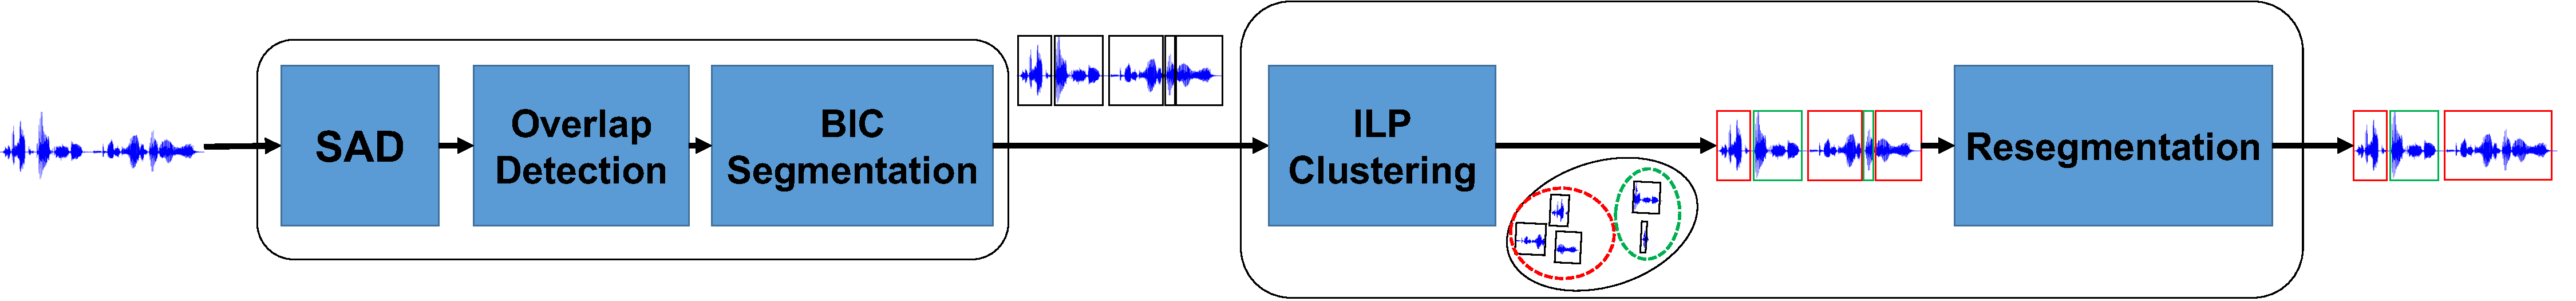
\includegraphics[height = 1in, width=1\textwidth]{figures/crssdiar_outline}
	\caption{\it \small CRSSDiar system overview. Two main steps are used in speaker diarization: 1) Segmentation (SAD, overlap detection, and BIC segmentation) and 2) clustering (ILP clustering and resegmentation). }
	\label{fig:crssdiar}
	\vspace{-3mm}
\end{figure}

\subsection{Interaction with Kaldi}
\label{ssec:crssdiar_and_kaldi}

As pointed at the beginning of the chapter, a driving force in developing this tool-kit was high compatibility with the Kaldi speech and speaker recognition platform~\cite{kaldi}. 
For those not familiar with the Kaldi project, it is a toolkit for speech recognition written in C++ and licensed under the Apache License v2.0. Kaldi is intended for use by speech recognition researchers~\cite{kaldi_doc}. 
Kaldi comprises many modules each designated to a specific task. For example, {\it feat} for feature extraction or {\it ivector} for ivector-based speaker recognition. 
Most modules come with a corresponding {\it bin} directory  that contains executable files used to perform various functions in a speech or speaker recognition system (e.g. {\it featbin}, {\it ivectorbin}). 
The executables are those most users interact with in their Bash scripts. These Bash scripts are also referred to as ``recipes''. 
CRSSDiar follows the same convention and consists of a {\it diar} and a {\it diarbin} directory. 
The classes are defined in {\it diar}, while {\it diarbin} contains the executables used to perform segmentation and clustering. 
CRSSDiar uses matrix and utility libraries from Kaldi in its core.  
Kaldi also includes modules that define Gaussian mixture models and Hidden Markov models ({\it gmm} and {\it hmm}), of which we also take advantage for acoustic modeling. 
As mentioned in the previous section, i-vectors are used in CRSSDiar as speaker-dependent features. 
Therefore, Kaldi's {\it ivector} is used to extract i-vectors and calculate distances and models such as PLDA\footnote{probabilistic linear discriminant analysis} to perform clustering. 
Figure~\ref{fig:crssdiar_vs_kaldi} shows the interaction between {\it diar} and {\it diarbin} components and Kaldi libraries. 

\begin{figure}[t!]
	\centering
	\textbf{CRSSDiar modules}\par\medskip
	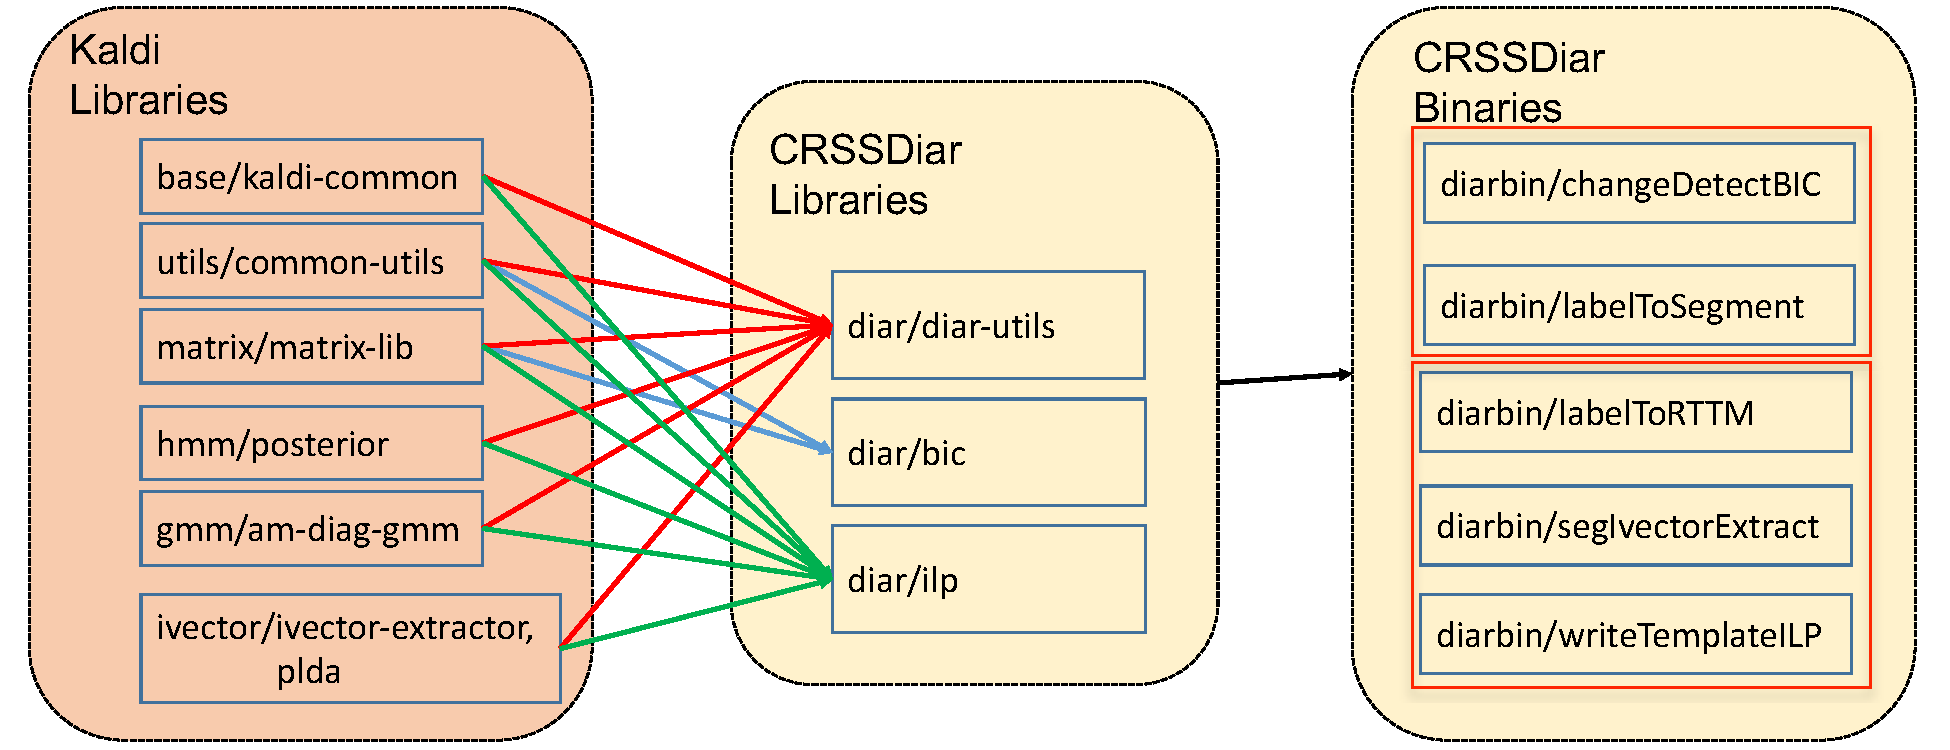
\includegraphics[height = 2in, width=0.8\textwidth]{figures/crssdiar_and_kaldi}
	\caption{\it \small CRSSDiar components and their relation with Kaldi libraries.  }
	\label{fig:crssdiar_vs_kaldi}
	\vspace{-3mm}
\end{figure}

\section{Segmentation}
\label{sec:segmentation}
This section briefly describes the layout of the Segmentation component in CRSSDiar. 
\section{Clustering}
\label{sec:clustering}